\section[Specific Requirements]{\hyperlink{toc}{Specific Requirements}}

\subsection[External Interface Requirements]{\hyperlink{toc}{External Interface Requirements}}
	\label{sec:externalInterfaceRequirements}
	%todo SafeStreets offers an interface to its customers to provide them its basic and advanced functionalities. All the data needed to authenticate the users will be managed inside the system as well as the information related to the violations in order to be mined and crossed whenever needed.
	\subsubsection[User Interfaces]{\hyperlink{toc}{User Interfaces}} % todo sistemare dimensioni mockups
	\label{sec:userInterfaces}
	The following section illustrates thanks to some mockups the interfaces SafeStreets provides to its customers in order to provide functionalities. Each picture is described only be the caption as complete and precise descriptions are given in the sections related to the description of the functionalities and how they are managed (\ref{sec:productFunctions}, \ref{sec:useCases}).
	
	\begin{figure}[h]
		\centering
		\begin{minipage}{0.45\textwidth}
			\centering
			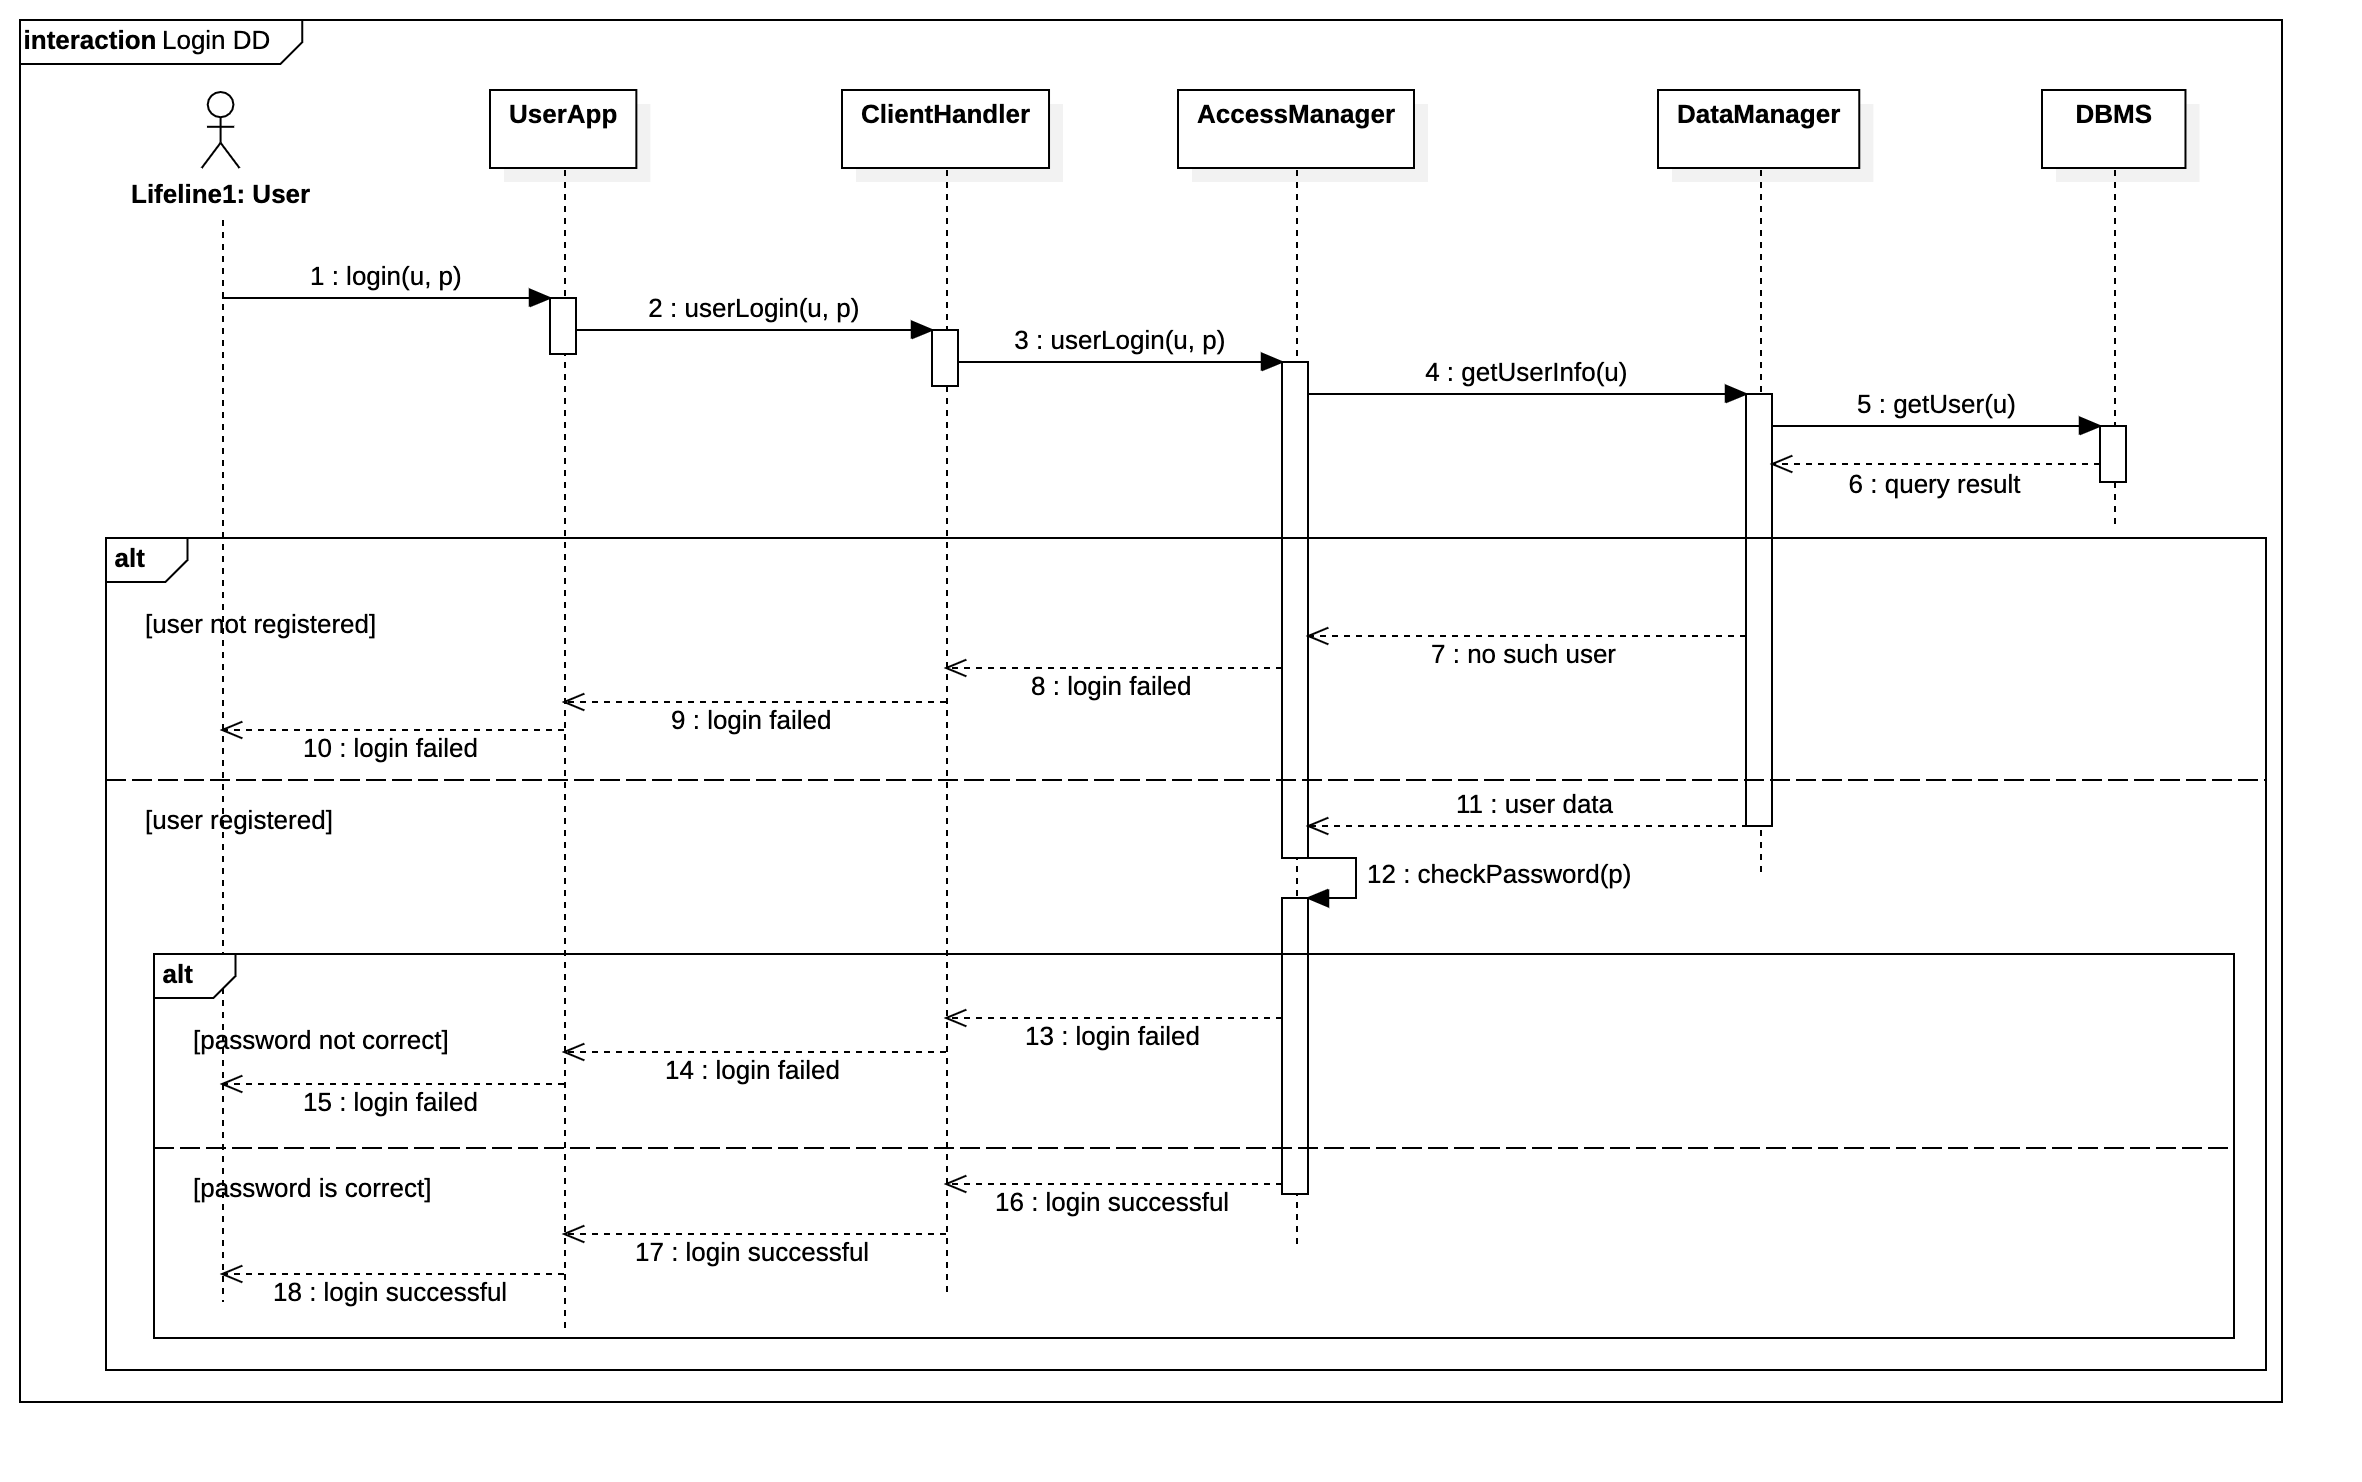
\includegraphics[width=0.58\textwidth]{/mockups/login.png}
			\caption{Login Interface}
		\end{minipage}\hfill
		\begin{minipage}{0.45\textwidth}
			\centering
			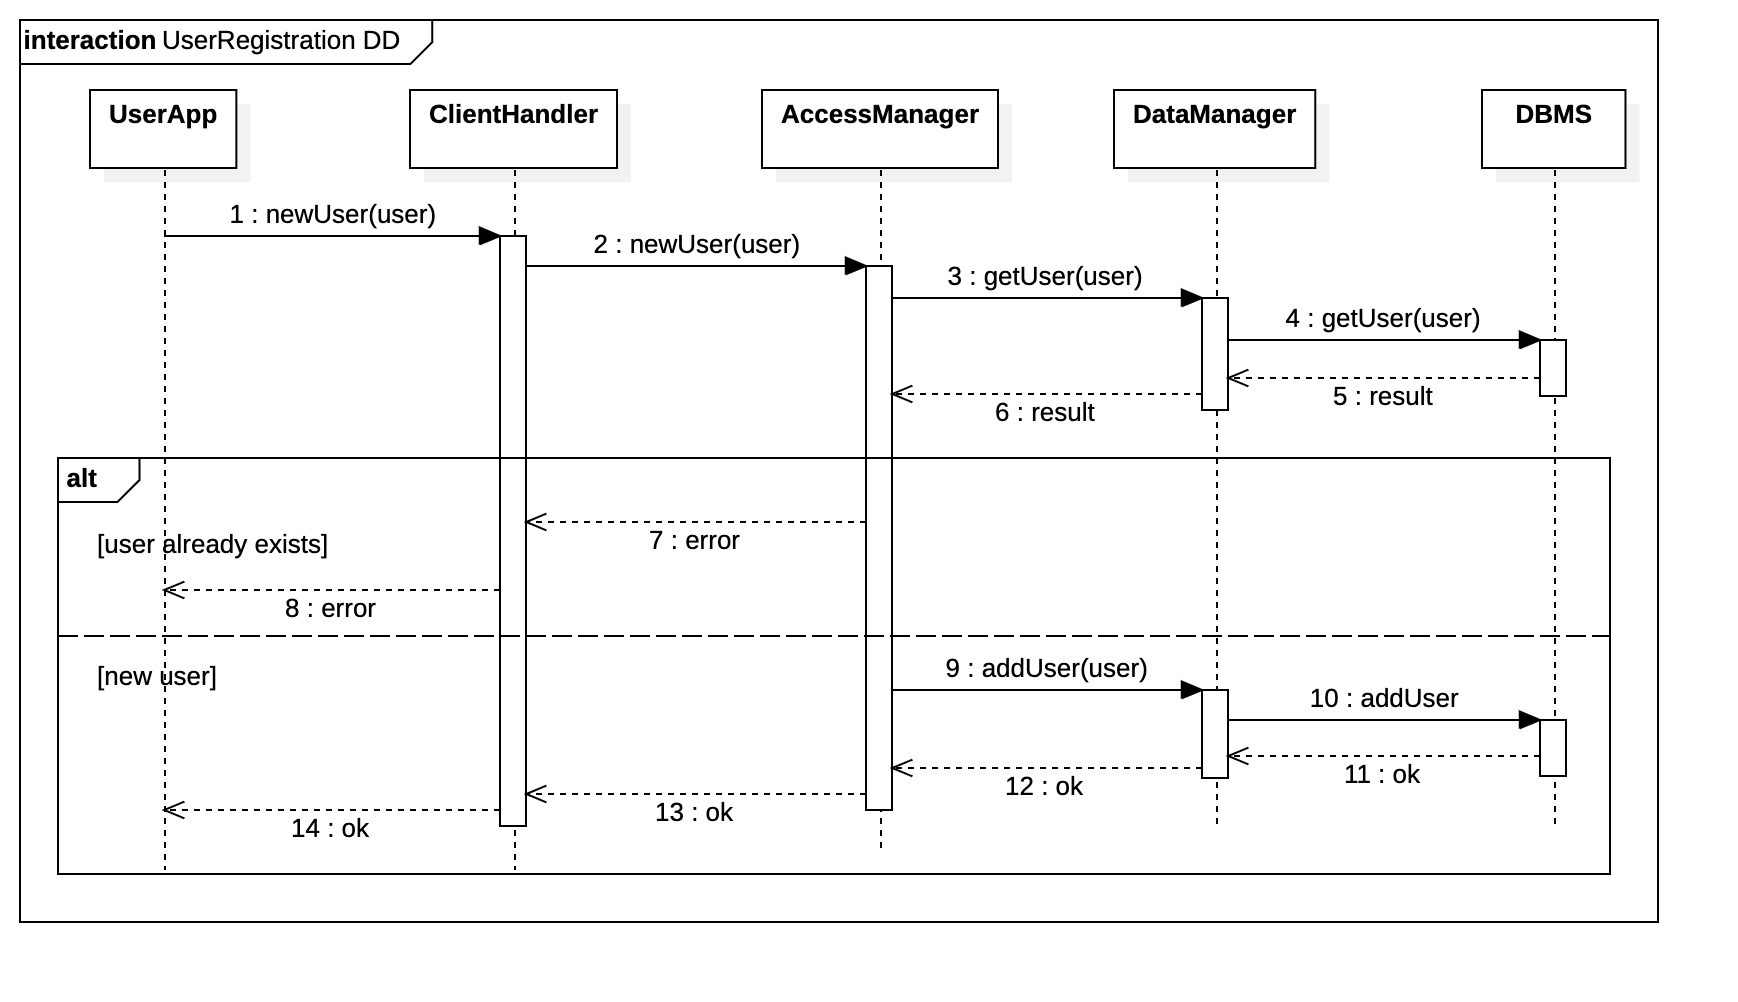
\includegraphics[width=0.58\textwidth]{/mockups/userRegistration.png}
			\caption{User Registration Interface}
		\end{minipage}
	\end{figure}

	\begin{figure}[h]
		\centering
		\begin{minipage}{0.45\textwidth}
			\centering
			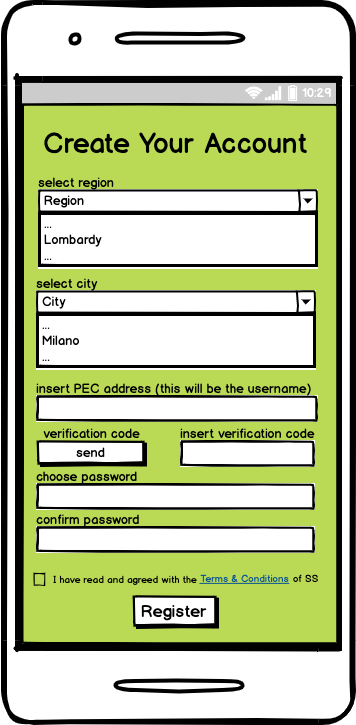
\includegraphics[width=0.58\textwidth]{/mockups/authorityRegistration.png}
			\caption{Authority Registration Interface}
		\end{minipage}\hfill
		\begin{minipage}{0.45\textwidth}
			\centering
			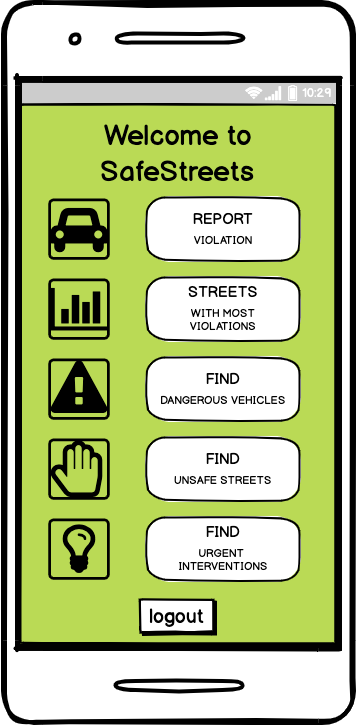
\includegraphics[width=0.58\textwidth]{/mockups/userHome.png}
			\caption{User Home Interface}
		\end{minipage}
	\end{figure}

	\begin{figure}[h]
		\centering
		\begin{minipage}{0.45\textwidth}
			\centering
			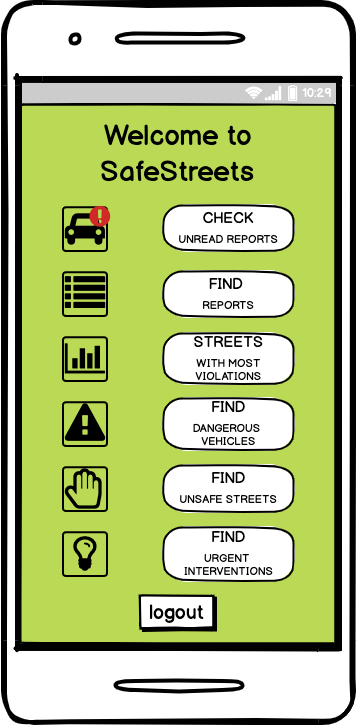
\includegraphics[width=0.7\textwidth]{/mockups/authorityHome.png}
			\caption{Authority Home Interface}
		\end{minipage}\hfill
		\begin{minipage}{0.45\textwidth}
			\centering
			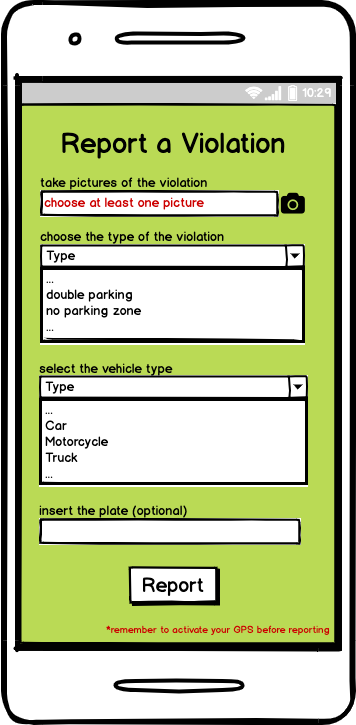
\includegraphics[width=0.7\textwidth]{/mockups/notification.png}
			\caption{Report Violation Interface}
		\end{minipage}
	\end{figure}

	\begin{figure}[h]
		\centering
		\begin{minipage}{0.45\textwidth}
			\centering
			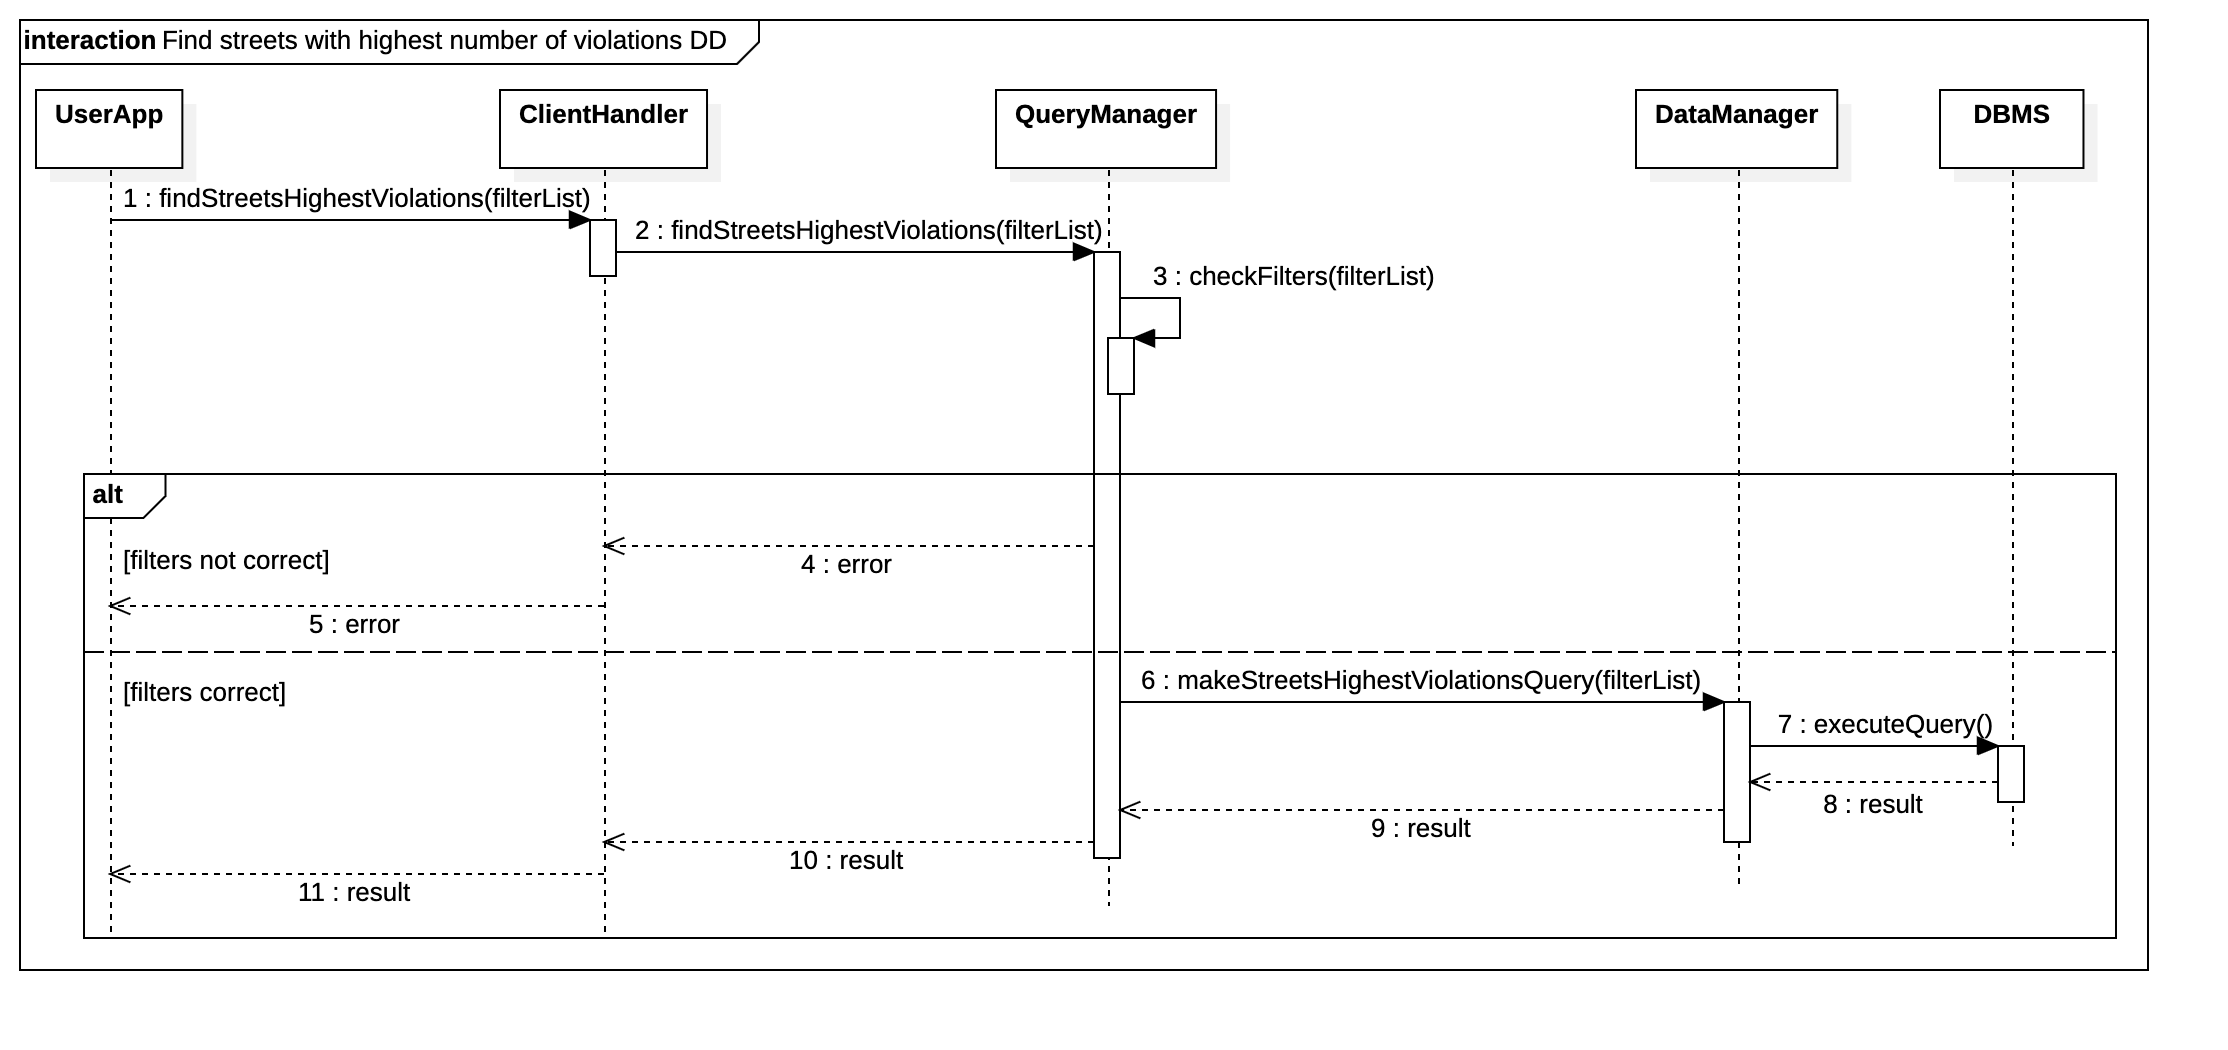
\includegraphics[width=0.7\textwidth]{/mockups/violationsFrequency.png}
			\caption{Streets With Most Violations Interface}
		\end{minipage}\hfill
		\begin{minipage}{0.45\textwidth}
			\centering
			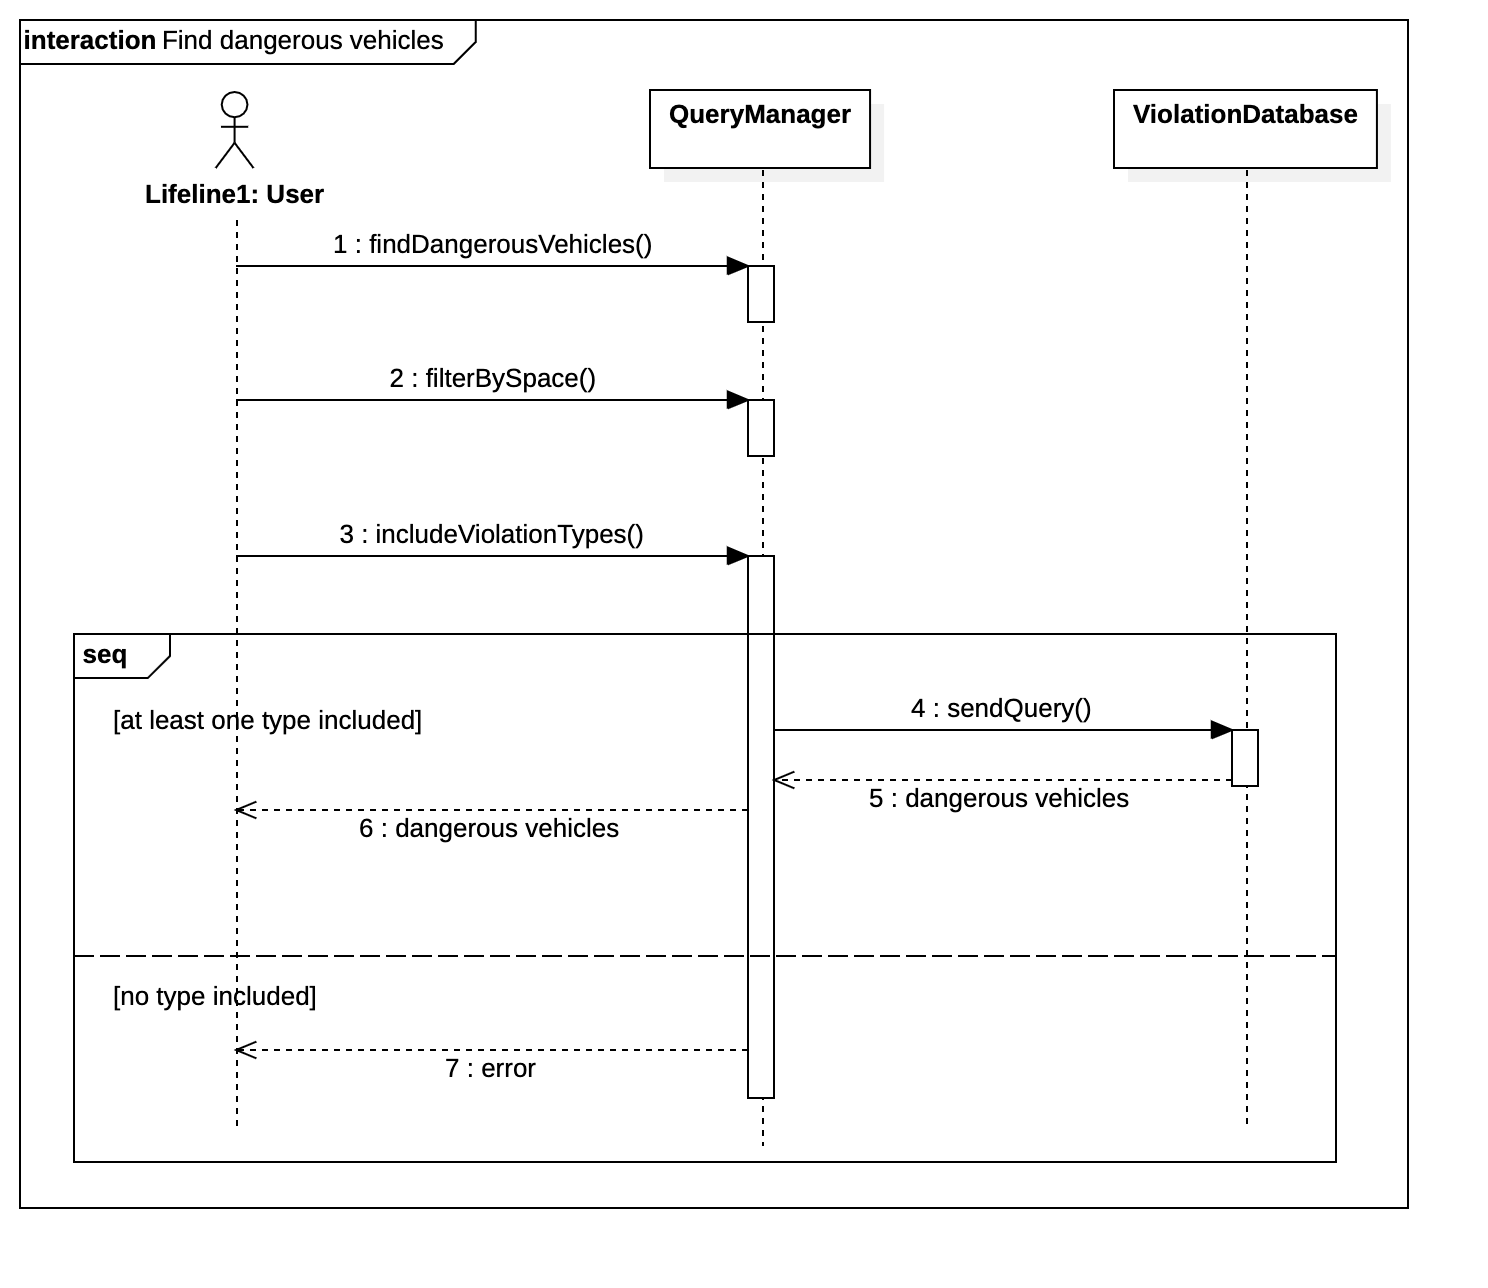
\includegraphics[width=0.7\textwidth]{/mockups/dangerousVehicles.png}
			\caption{Dangerous Vehicles Interface}
		\end{minipage}
	\end{figure}

	\begin{figure}[h]
		\centering
		\begin{minipage}{0.45\textwidth}
			\centering
			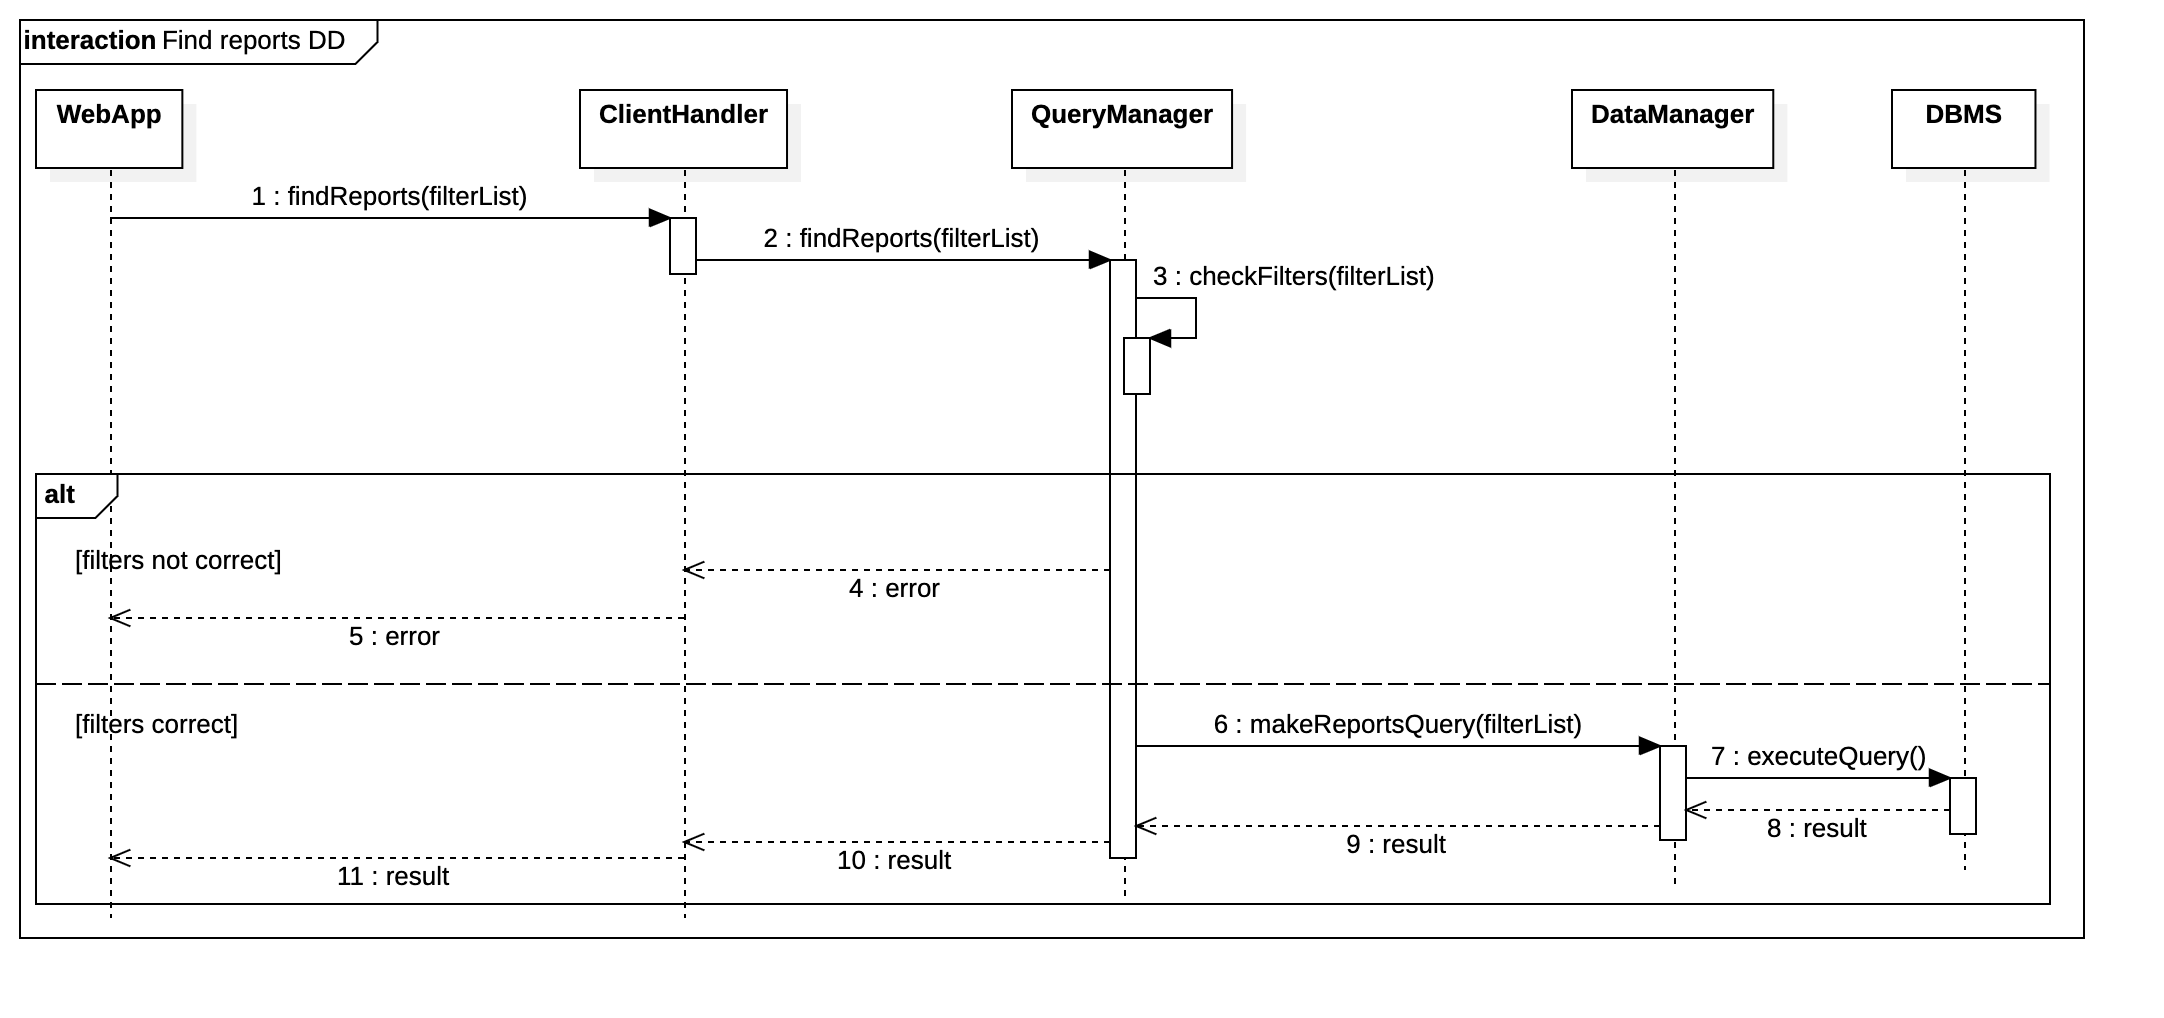
\includegraphics[width=0.7\textwidth]{/mockups/findReports.png}
			\caption{Find Reports Interface}
		\end{minipage}\hfill
		\begin{minipage}{0.45\textwidth}
			\centering
			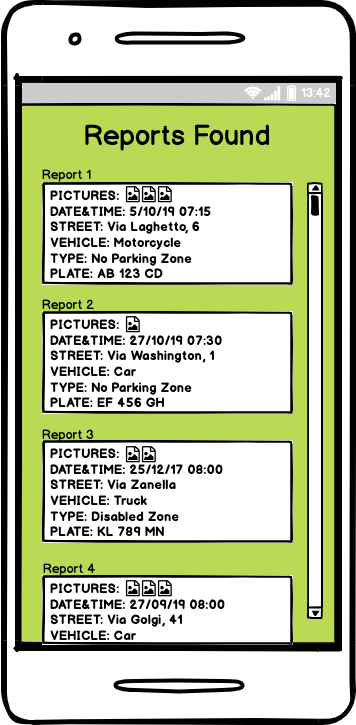
\includegraphics[width=0.7\textwidth]{/mockups/reportsFound.png}
			\caption{Reports Found Interface Result}
		\end{minipage}
	\end{figure}

	\begin{figure}[h]
		\centering
		\begin{minipage}{0.45\textwidth}
			\centering
			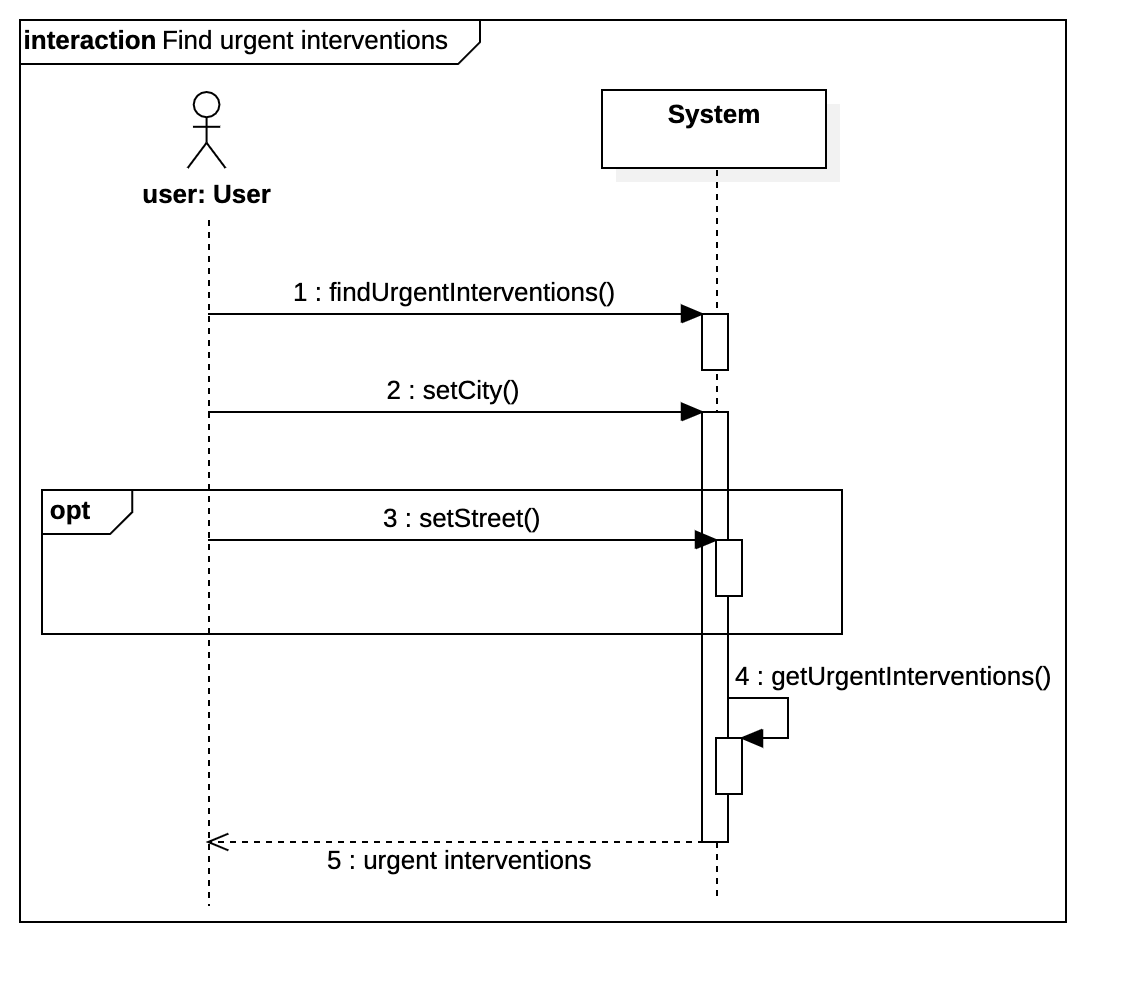
\includegraphics[width=0.7\textwidth]{/mockups/urgentInterventions.png}
			\caption{Urgent Interventions Interface}
		\end{minipage}\hfill
		\begin{minipage}{0.45\textwidth}
			\centering
			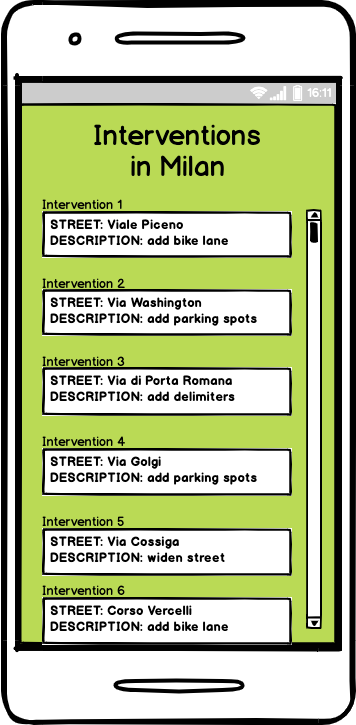
\includegraphics[width=0.7\textwidth]{/mockups/interventionsFound.png}
			\caption{Intervention Found Interface Result}
		\end{minipage}
	\end{figure}
	 
	 \begin{figure}[h]
	 	\centering
	 	\begin{minipage}{0.45\textwidth}
	 		\centering
	 		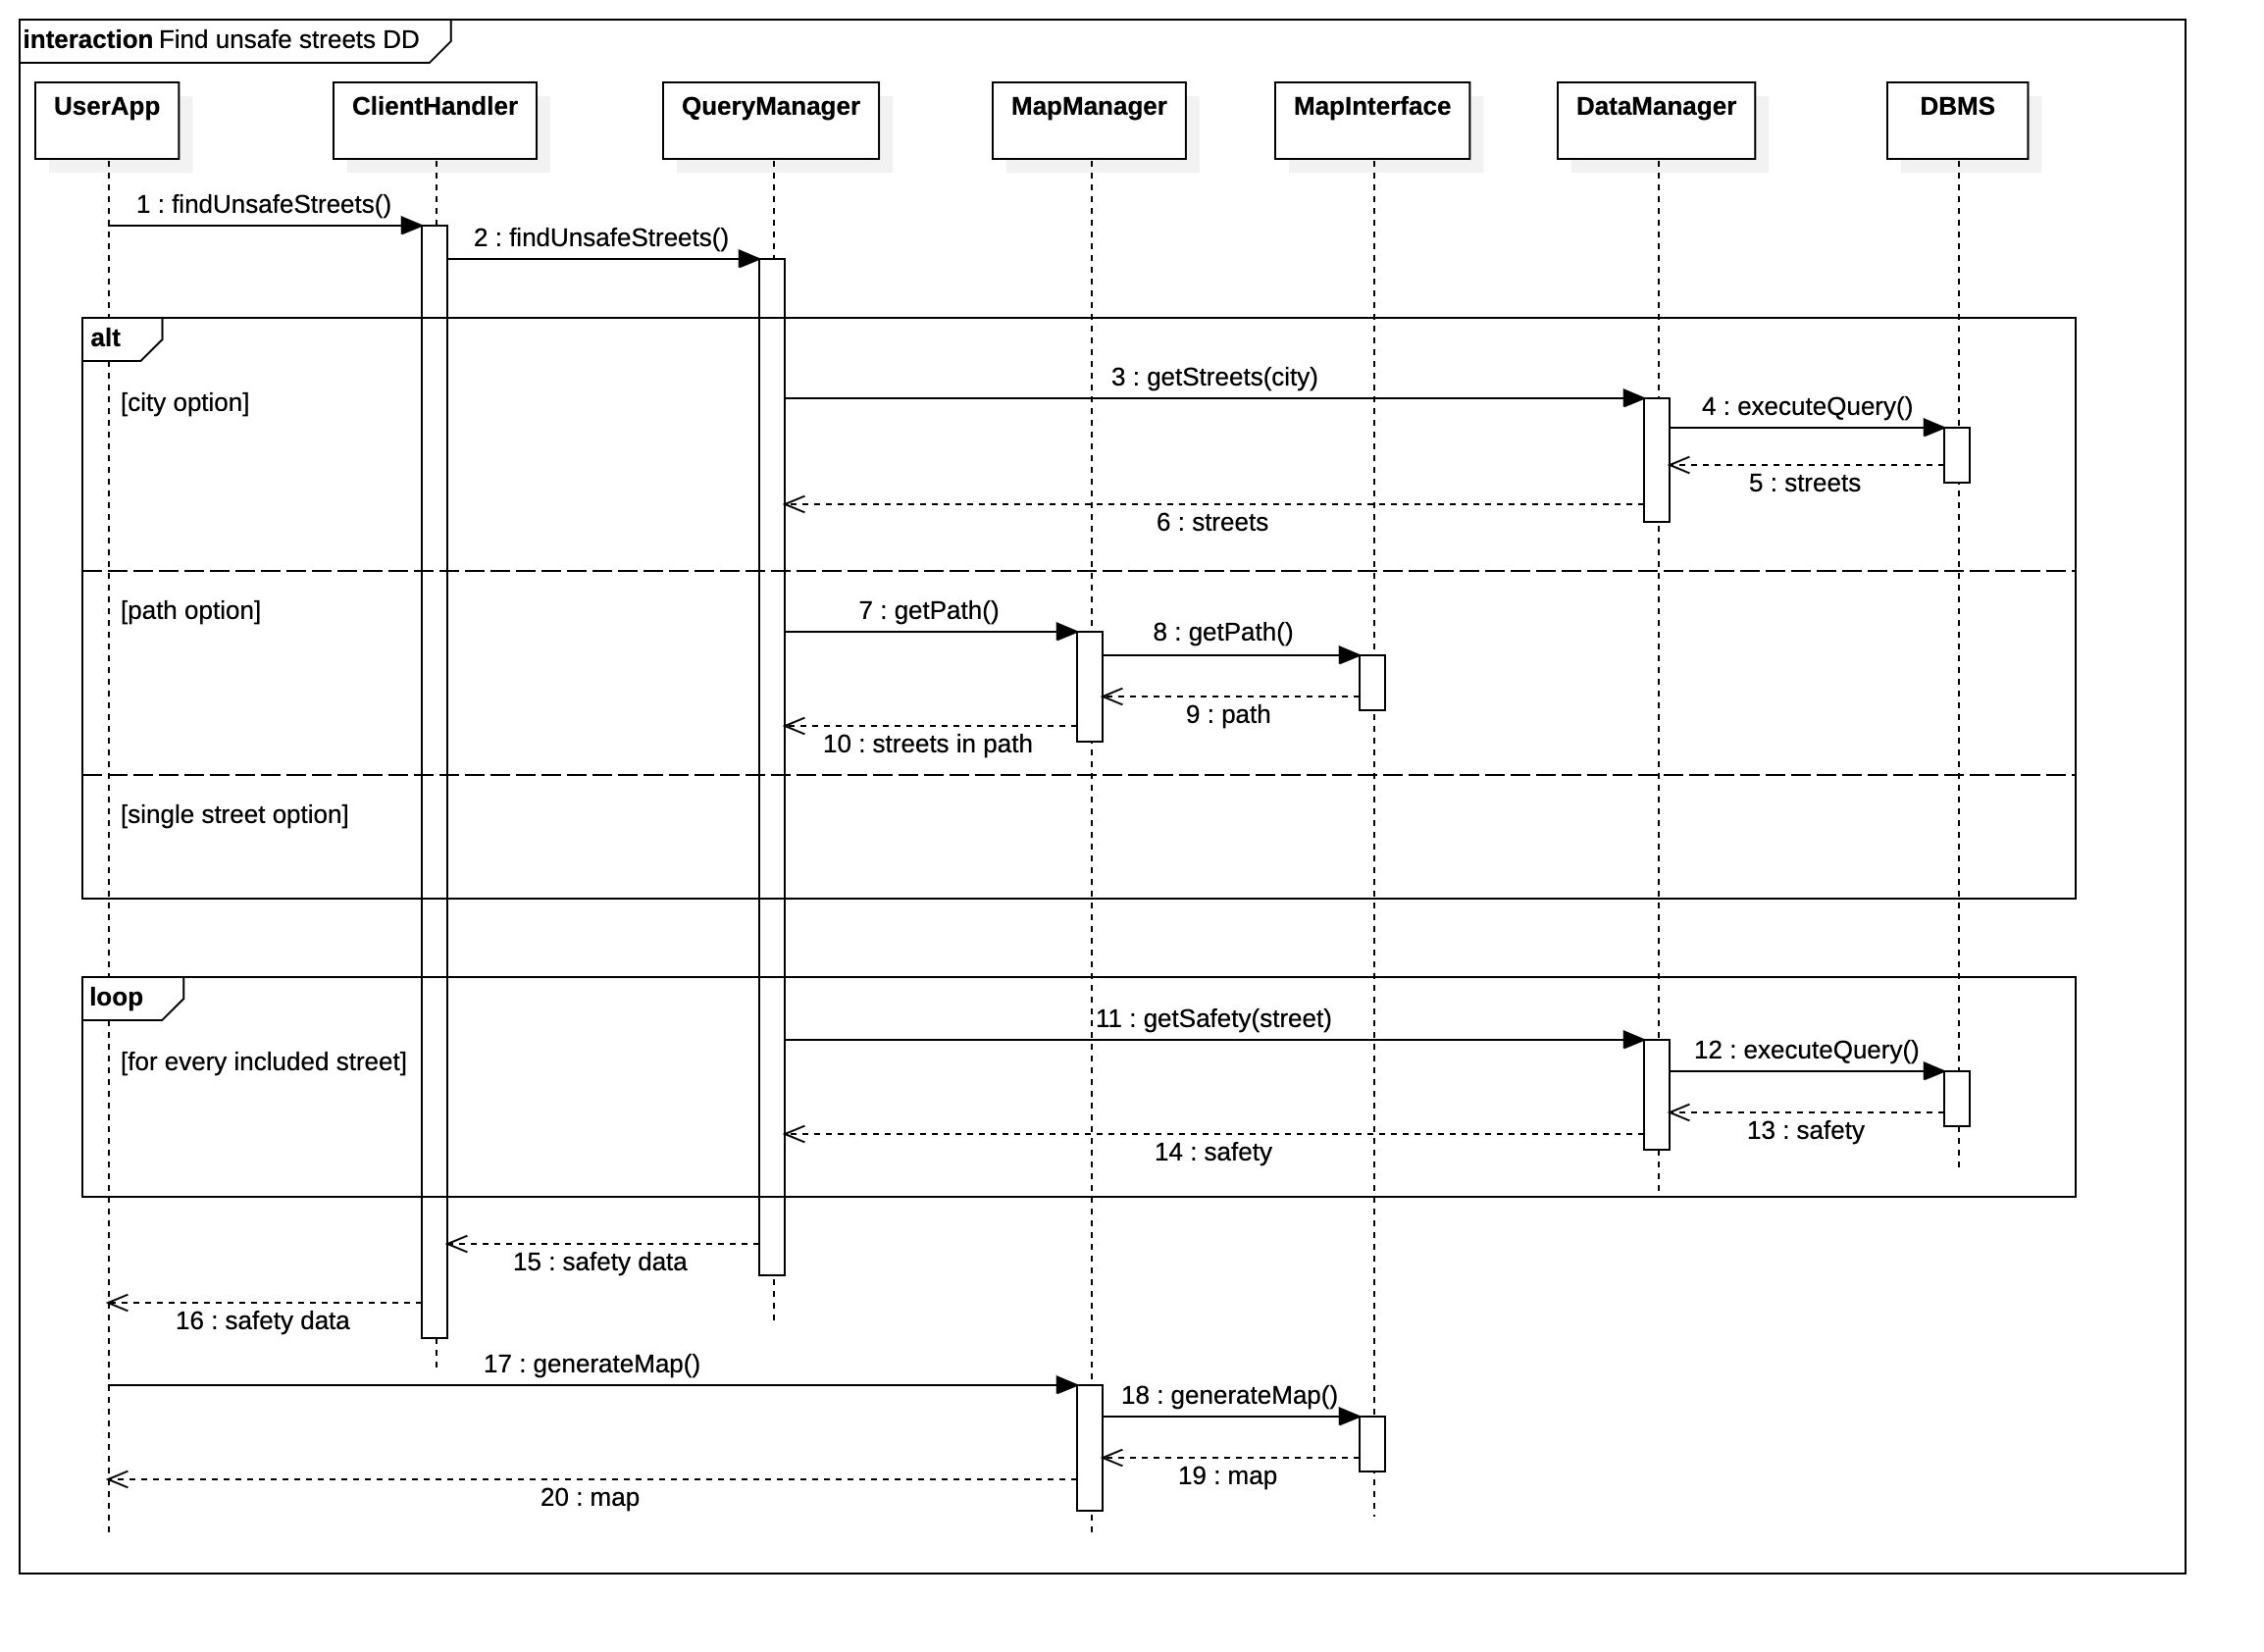
\includegraphics[width=0.7\textwidth]{/mockups/unsafeStreets.png}
	 		\caption{Streets Safety Interface}
	 	\end{minipage}
 		\begin{minipage}{0.45\textwidth}
 			
 		\end{minipage}
	 \end{figure} 
	\FloatBarrier
	\subsubsection[Hardware Interfaces]{\hyperlink{toc}{Hardware Interfaces}}
	\subsubsection[Software Interfaces]{\hyperlink{toc}{Software Interfaces}}
	\subsubsection[Communication Interfaces]{\hyperlink{toc}{Communication Interfaces}}

\subsection[Functional Requirements]{\hyperlink{toc}{Functional Requirements}}

\subsubsection[Use Cases Diagrams]{\hyperlink{toc}{Use Cases Diagrams}}

\subsubsection[Use Cases Description]{\hyperlink{toc}{Use Cases Description}}
	\label{sec:useCases}
	
	\paragraph{User}
	\begin{enumerate}
		\item \textbf{User Registration} 
			\begin{longtable}{p{0.25\linewidth}p{0.75\linewidth}}
				\toprule
				\textbf{Name} & \textbf{User Registration} \\
				\midrule
				\textbf{Actors} & User \\
				\midrule
				\textbf{Entry conditions} & The application has started \\
				\midrule
				\textbf{Flow of events} & 
				\begin{enumerate}
					\item The user chooses the sign up option
					\item The user selects the 'user' registration type
					\item The user chooses a username and a password
					\item The user inserts his name, surname and address
					\item The user submits the form
					\item The system checks the username to be unique
					\item The system saves the user data
				\end{enumerate} \\
				\midrule
				\textbf{Exit conditions} & The user is registered in the system\\
				\midrule
				\textbf{Exceptions} & 
				\begin{itemize}
					\item If the username inserted by the user is already used by another user, or if the username contains any special character, the system displays an error message asking the user to insert a different one
				\end{itemize} \\
				\bottomrule
				\caption{\emph{User Registration} use case description}
			\end{longtable}
		
		\item \textbf{User Login}
			\begin{longtable}{p{0.25\linewidth}p{0.75\linewidth}}
				\toprule
				\textbf{Name} & \textbf{User Login} \\
				\midrule
				\textbf{Actors} & User \\
				\midrule
				\textbf{Entry conditions} & The application has started \\
				\midrule
				\textbf{Flow of events} & 
				\begin{enumerate}
					\item The user chooses the login option
					\item The user chooses the 'user' login type
					\item The user inserts his username
					\item The user inserts his password
					\item The user submits the form
					\item The system checks the username to be existing
					\item The system checks the password to be right for that username
					\item The system notifies the user that login is successful
				\end{enumerate} \\
				\midrule
				\textbf{Exit conditions} & The user is logged in\\
				\midrule
				\textbf{Exceptions} & 
				\begin{itemize}
					\item If the username is not recognized by the system, that means that the user is not registered yet, or the username is incorrect. The system notifies the user and the procedure is aborted
					\item If the inserted password is wrong, the system notifies the user and the procedure is aborted			
				\end{itemize} \\
				\bottomrule
				\caption{\emph{User Login} use case description}
			\end{longtable}
		
		\item \textbf{Report Violation}
			\begin{longtable}{p{0.25\linewidth}p{0.75\linewidth}}
				\toprule
				\textbf{Name} & \textbf{Report violation} \\
				\midrule
				\textbf{Actors} & User \\
				\midrule
				\textbf{Entry conditions} & The user is logged in \\
				\midrule
				\textbf{Flow of events} & 
				\begin{enumerate}
					\item The user selects the report violation option
					\item The system retrieves the GPS location
					\item The user chooses the option to take pictures
					\item The user takes some pictures through the application
					\item The user selects the pictures he wants to send
					\item The user optionally inserts the license plate number
					\item The user chooses the type of violation from a list
					\item The user chooses the type of vehicle from a list
					\item The user chooses the option to confirm
					\item The system receives the sent data
					\item The system runs an algorithm to read the license plate, with the help of the information provided by the user
					\item The system retrieves the name of the street from the GPS location
					\item The system stores the violation report
				\end{enumerate} \\
				\midrule
				\textbf{Exit conditions} & The information about the violation is stored\\
				\midrule
				\textbf{Exceptions} & 
				\begin{itemize}
					\item If the system fails to retrieve the GPS location, the user is notified and the application shows the home page
					\item If the system fails to read the license plate, or what it reads does not match the information provided by the user, the field will be left empty
				\end{itemize} \\
				\bottomrule
				\caption{\emph{Report violation} use case description}
			\end{longtable}
		
		\item \textbf{Find streets with the highest number of violations}
			\begin{longtable}{p{0.25\linewidth}p{0.75\linewidth}}
				\toprule
				\textbf{Name} & \textbf{Find streets with the highest number of violations} \\
				\midrule
				\textbf{Actors} & User \\
				\midrule
				\textbf{Entry conditions} & The user is logged in \\
				\midrule
				\textbf{Flow of events} & 
				\begin{enumerate}
					\item The user selects the 'streets with highest number of violation' option
					\item The user chooses the region he is looking for from a list
					\item The user chooses the city from a list
					\item The user chooses the types of violation to be included
					%maybe a checkbox
					\item The user chooses the time slot
					\item The user chooses the types of vehicle to be included
					\item The user confirms the query and sends it
					\item The system returns a list of the streets ordered by the highest number of violations, with the actual number next to the name of the street, according to the filters
				\end{enumerate} \\
				\midrule
				\textbf{Exit conditions} & The list of the streets is shown to the user \\
				\midrule
				\textbf{Exceptions} & 
				\begin{itemize}
					\item 	If no type of violation is selected, the system shows an error message and the procedure is aborted
					\item If no type of vehicle is selected, the system shows an error message and the procedure is aborted	
				\end{itemize} \\
				\bottomrule
				\caption{\emph{Find streets with the highest number of violations} use case description}
			\end{longtable}
		
		\item \textbf{Find Most Dangerous Vehicles}
			\begin{longtable}{p{0.25\linewidth}p{0.75\linewidth}}
				\toprule
				\textbf{Name} & \textbf{Find dangerous vehicles} \\
				\midrule
				\textbf{Actors} & User \\
				\midrule
				\textbf{Entry conditions} & The user is logged in \\
				\midrule
				\textbf{Flow of events} & 
				\begin{enumerate}
					\item The user selects the 'most dangerous vehicles' option
					\item The user selects the region and the city from a list, or selects a street, or selects everywhere
					\item The user selects the types of violation he wants to include
					\item The user confirms the query and sends it
					\item The system returns a list of the types of vehicle, ordered by the highest number of violations they committed, according to the filters
				\end{enumerate} \\
				\midrule
				\textbf{Exit conditions} & The list is shown to the user\\
				\midrule
				\textbf{Exceptions} & 
				\begin{itemize}
					\item 	If no type of violation is selected, the system notifies the user and wait for him to insert at least one	
				\end{itemize} \\
				\bottomrule
				\caption{\emph{Find most dangerous vehicles} use case description}
			\end{longtable}
		
		\item \textbf{Find Urgent Interventions}
			\begin{longtable}{p{0.25\linewidth}p{0.75\linewidth}}
				\toprule
				\textbf{Name} & \textbf{Find urgent interventions} \\
				\midrule
				\textbf{Actors} & User \\
				\midrule
				\textbf{Entry conditions} & The user is logged in \\
				\midrule
				\textbf{Flow of events} & 
				\begin{enumerate}
					\item The user selects the 'urgent interventions' option
					\item The user selects the region and the city from a list
					%todo Magari facciamo anche filtrare per tipi di interventions
					\item The user confirms the query and sends it
					\item The system returns a list of the most urgent interventions in the selected city, each with their respective street
					%todo comunque in qualche modo i tipi di intervento vanno modellati
				\end{enumerate} \\
				\midrule
				\textbf{Exit conditions} & The list is shown to the user\\
				\midrule
				\textbf{Exceptions} &  \\
				\bottomrule
				\caption{\emph{Find urgent interventions} use case description}
			\end{longtable}
		
		\item \textbf{Find Unsafe Streets}
			\begin{longtable}{p{0.25\linewidth}p{0.75\linewidth}}
				\toprule
				\textbf{Name} & \textbf{Find unsafe streets} \\
				\midrule
				\textbf{Actors} & User \\
				\midrule
				\textbf{Entry conditions} & The user is logged in \\
				\midrule
				\textbf{Flow of events} & 
				\begin{enumerate}
					%todo ma quanto bisogna specificare quello che fa il sistema in tutto questo?
					\item The user selects the 'unsafe streets' option
					\item The user selects the either the 'city' option, the 'route' option or the single street option
					\item The user chooses the region and the city from a list if 'city' option is chosen, if 'route' option is chosen he enters start and end points of the route, otherwise he inserts the name of the street
					\item The user confirms the query and sends it
					\item The system returns a map where the streets selected with the filter are colored according to their safety: green if they're 'safe', red if they're 'unsafe'
				\end{enumerate} \\
				\midrule
				\textbf{Exit conditions} & The list is shown to the user\\
				\midrule
				\textbf{Exceptions} & 
				\begin{itemize}
					\item If no city is selected when 'city' option is chosen, the system notifies the user and waits for him to insert it
					\item If no start or end points are chosen when 'route' option is selected, the system notifies the user and waits for him to insert them
				\end{itemize} \\
				\bottomrule
				\caption{\emph{Find unsafe streets} use case description}
			\end{longtable}
	\end{enumerate}
		
	\paragraph{Authority}
	\begin{enumerate}
		\item \textbf{Authority Registration}
			\begin{longtable}{p{0.25\linewidth}p{0.75\linewidth}}
				\toprule
				\textbf{Name} & \textbf{Registration} \\
				\midrule
				\textbf{Actors} & Authority \\
				\midrule
				\textbf{Entry conditions} & The application has started \\
				\midrule
				\textbf{Flow of events} & 
				\begin{enumerate}
					\item The authority chooses the sign up option
					\item The authority selects the 'authority' registration type
					\item The authority chooses the region and the city of competence
					\item The authority inserts its PEC address
					\item The system checks that PEC address matches the chosen city
					\item The system sends a confirmation code to the PEC address
					\item The authority enters the confirmation code in a text box
					\item The authority submits the form
					\item The system checks the entered code to match the sent one
					\item The system saves the authority's data
				\end{enumerate} \\
				\midrule
				\textbf{Exit conditions} & The authority is registered in the system\\
				\midrule
				\textbf{Exceptions} & 
				\begin{itemize}
					\item If the selected city already has an authority registered, an error message is shown and the procedure is aborted
					\item If the PEC address doesn't match the chosen city, an error message is shown and the procedure is aborted
					\item If the entered code doesn't match the sent one, an error message is shown and the procedure is aborted
				\end{itemize} \\
				\bottomrule
				\caption{\emph{Authority Registration} use case description}
			\end{longtable}
		
		\item \textbf{Authority Login}
			\begin{longtable}{p{0.25\linewidth}p{0.75\linewidth}}
				\toprule
				\textbf{Name} & \textbf{Authority Login} \\
				\midrule
				\textbf{Actors} & Authority\\
				\midrule
				\textbf{Entry conditions} & The application has started \\
				\midrule
				\textbf{Flow of events} & 
				\begin{enumerate}
					\item The authority chooses the login option
					\item The authority chooses the 'authority' login type
					\item The authority inserts its PEC address as username
					\item The authority inserts its password
					\item The authority submits the form
					\item The system checks the username to be registered
					\item The system checks the password to be right for that username
					\item The system notifies the authority that login is successful
				\end{enumerate} \\
				\midrule
				\textbf{Exit conditions} & The authority is logged in\\
				\midrule
				\textbf{Exceptions} & 
				\begin{itemize}
					\item If the username is not recognized by the system, that means that the authority is not registered yet, or the username is incorrect. The system notifies the authority and the procedure is aborted
					\item If the inserted password is wrong, the system notifies the authority and the procedure is aborted			
				\end{itemize} \\
				\bottomrule
				\caption{\emph{Authority Login} use case description}
			\end{longtable}
		
		\item \textbf{Check Unread Reports}
			\begin{longtable}{p{0.25\linewidth}p{0.75\linewidth}}
				\toprule
				\textbf{Name} & \textbf{Check unread reports} \\
				\midrule
				\textbf{Actors} & Authority\\
				\midrule
				\textbf{Entry conditions} & The authority is logged in \\
				\midrule
				\textbf{Flow of events} & 
				\begin{enumerate}
					\item The authority chooses the 'unread reports' option
					\item The system provides a list with all the unread violation reports that match the city of competence of the authority
				\end{enumerate} \\
				\midrule
				\textbf{Exit conditions} & The list is shown to the authority\\
				\midrule
				\textbf{Exceptions} &  \\
				\bottomrule
				\caption{\emph{Check unread reports} use case description}
			\end{longtable}
			
		\item \textbf{Find Reports}
			\begin{longtable}{p{0.25\linewidth}p{0.75\linewidth}}
				\toprule
				\textbf{Name} & \textbf{Find reports} \\
				\midrule
				\textbf{Actors} & Authority\\
				\midrule
				\textbf{Entry conditions} & The authority is logged in \\
				\midrule
				\textbf{Flow of events} & 
				\begin{enumerate}
					\item The authority chooses the 'find reports' option
					\item The authority selects the types of violation to be included
					\item The authority selects date interval and time slot
					\item The authority selects the types of vehicle to be included
					\item The authority optionally selects the street to include, otherwise 'city' will be selected
					\item The authority confirms and sends the query
					\item The system provides a list with all the violation reports that match the filter, sorted by chronological order from the most recent one. In case 'city' option is selected, the considered city is that of competence of the authority
				\end{enumerate} \\
				\midrule
				\textbf{Exit conditions} & The list is shown to the authority\\
				\midrule
				\textbf{Exceptions} &  
				\begin{enumerate}
					\item If the date interval is not valid, the system notifies the authority and the procedure is aborted
				\end{enumerate}\\
				\bottomrule
				\caption{\emph{Find reports} use case description}
			\end{longtable}
	\end{enumerate}

\subsubsection[Traceability Matrix]{\hyperlink{toc}{Traceability Matrix}} % aggiungi le c nella tabular e i requirements per aumentare le dimensioni, c line anche il 9 è il numero di colonne cambia anche quello così si copre bene tutta la tabella
	\begin{tabular}{|c|c|c|c|c|c|c|c|c|}
		\cline{2-9}
		\multicolumn{1}{c|}{} & R1 & R2 & R3 & R4 & R5 & R6 & R7 & R8 \\
		\hline
		use case 1 & \xmark & & & & & & &\\
		\hline
		use case 2 & & & & \xmark & & & &\\
		\hline
		use case 3 & \xmark & \xmark & \xmark & & & & \xmark &\\
		\hline
	\end{tabular}
	
\subsection[Performance Requirements]{\hyperlink{toc}{Performance Requirements}}

\subsection[Design Constraints]{\hyperlink{toc}{Design Constraints}}
	\subsubsection[Standards Compliance]{\hyperlink{toc}{Standards Compliance}}
	\subsubsection[Hardware Limitations]{\hyperlink{toc}{Hardware Limitations}}
	\subsubsection[Any other Constraint]{\hyperlink{toc}{Any other Constraint}}

\subsection[Software System Attributes]{\hyperlink{toc}{Software System Attributes}}
	\subsubsection[Reliability]{\hyperlink{toc}{Reliability}}
	\subsubsection[Availability]{\hyperlink{toc}{Availability}}
	\subsubsection[Security]{\hyperlink{toc}{Security}}
	\subsubsection[Maintainability]{\hyperlink{toc}{Maintainability}}
	\subsubsection[Portability]{\hyperlink{toc}{Portability}}
